\documentclass[12pt, a4paper]{article}


% --- 核心宏包 ---
\usepackage{graphics}
\usepackage{float}
\usepackage[UTF8]{ctex}        % 中文支持
%\usepackage[UTF8]{inputenc}
\usepackage{geometry}         % 页面边距
\usepackage{graphicx}         % 插入图片
\usepackage{amsmath, amssymb} % 数学公式
\usepackage{setspace}         % 行间距
\usepackage{titlesec}         % 标题格式定制
\usepackage{booktabs}         % 三线表（推荐用于性能评估报告）
\usepackage{hyperref}         % 超链接
\usepackage[backend=biber, style=gb7714-2015]{biblatex} % 使用国标格式
\addbibresource{refs.bib} % 导入refs文件
% --- 页面设置 ---
\geometry{left=3.18cm, right=3.18cm, top=2.54cm, bottom=2.54cm} % 类似Word标准页边距
\onehalfspacing % 1.5倍行距 

% --- 标题格式设置 (符合模板要求) ---
\titleformat{\section}{\large\bfseries}{\thesection}{1em}{}
\titleformat{\subsection}{\normalsize\bfseries}{\thesubsection}{1em}{}

\begin{document}


% --- 封面简版 (手动排版，不使用 \maketitle) ---
\begin{center}
	
\includegraphics[width=0.8\textwidth]{figures/XJTU_2024.png}
	\vspace*{1.5cm}
	\newline
	{\LARGE \textbf{低功耗Int8数字存算一体架构设计与FPGA验证（开题）}} \\[2cm]

	\vspace*{3cm}

	\begin{spacing}{2.0}
		\begin{tabular}{ll}
			\textbf{学 \quad 号：} & 2221411116                                                                   \\
			\textbf{姓 \quad 名：} & 焦宏宝                                                                          \\
			\textbf{导 \quad 师：} & 梁峰                                                                           \\
			\textbf{论文题目：}      & \begin{tabular}[t]{l} 面向边缘智能应用的低功耗Int8 -- \\ 数字存算一体架构设计及FPGA验证 \end{tabular} \\
			\textbf{专 \quad 业：} & 微电子科学与工程 强芯实验班                                                               \\
			\textbf{学 \quad 院：} & 电信学部　微电子学院                                                                   \\
			\textbf{填写时间：}      & 2026年 01月
		\end{tabular}
	\end{spacing}
\end{center}

\newpage

% --- 目录 ---
\tableofcontents
\newpage

% --- 正文开始 ---

\section{选题的背景及依据}
\subsection{选题背景}
近年来，以 YOLO\cite{10}、SSD\cite{11} 为代表的深度学习目标检测算法在智能安防、工业视觉、无人系统与车载感知等场景中被广泛采用，其共同特点是需要在较高精度下实现接近实时的推理能力，而网络内部又以卷积/矩阵乘加（MAC）为主导计算负载，导致整体计算量与数据访问量都十分庞大。YOLO 将检测任务端到端地建模为单网络回归问题，SSD 通过多尺度特征图上的卷积预测实现单阶段检测，这类方法在追求速度与精度的同时，也使得卷积算子成为系统性能与功耗优化的核心瓶颈之一。


\begin{figure}[H]
	\centering
	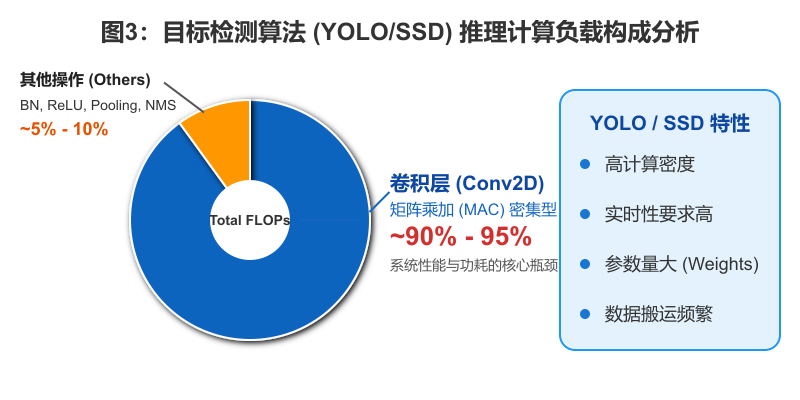
\includegraphics[width=0.8\textwidth]{figures/3.png}
\end{figure}

然而，在传统冯·诺依曼架构中，处理器与存储器相互分离，权重与特征图等数据需要在存储层级与计算单元之间频繁搬运，系统性能逐渐受限于存储带宽与访问延迟，“内存墙（Memory Wall）”问题由此形成并长期存在。Wulf 与 McKee 早在 1995 年就指出处理器速度提升与存储器速度提升之间的差距会不断扩大，从而限制系统级性能提升\cite{1}。与此同时，能效维度的矛盾更加突出：在先进工艺条件下，数据搬运（尤其是跨层级、跨片外存储访问）相对于算术运算存在显著更高的能量代价，使得“算得快”并不等价于“算得省”。Horowitz 在 ISSCC 2014 的报告中系统讨论了计算系统的能耗拆分，强调需要从体系结构与数据流层面减少昂贵的数据访问\cite{2}。面向 CNN 的专用加速器研究也进一步表明：通过数据复用与数据流优化降低（尤其是片外）访存开销，是实现低功耗实时推理的关键路径之一\cite{3}。在边缘计算场景（电池供电、散热受限、实时性要求高）中，上述矛盾更加尖锐，传统“分离式计算-存储”模式难以同时满足吞吐与能效需求。

\begin{figure}[H]
	\centering
	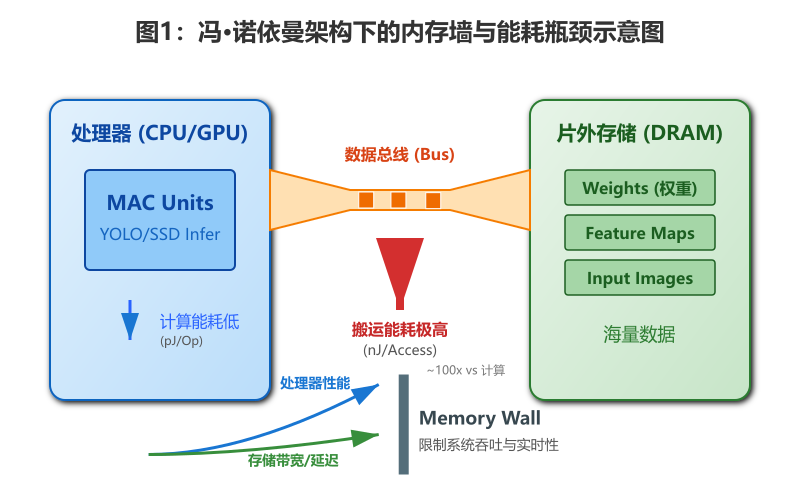
\includegraphics[width=0.8\textwidth]{figures/1.png}
\end{figure}



存算一体（Computing-in-Memory, CIM）技术通过在存储阵列内部或近存储位置完成计算，将“数据搬运”转化为“原位计算”，从体系结构层面缓解冯·诺依曼瓶颈，被认为是突破内存墙、提升能效与吞吐率的重要方向。Nature Electronics 的综述工作提出了覆盖不同存储器参与程度的 CIM 全谱系分类框架，并指出 CIM 可在逻辑运算与乘加运算等基本原语上实现能效提升\cite{4}。在诸多实现路径中，基于标准 CMOS 工艺的 SRAM-CIM 具有速度快、工艺成熟、可靠性高、与主流数字设计流程兼容等优点，是面向工程落地与系统集成的重要路线之一；相关综述也指出 SRAM-CIM 在电路、功能与应用层面持续演进，逐步从低比特/简单算子走向更高精度、更贴近 DNN 推理的计算形态\cite{5}。

从应用角度看，为在精度、硬件复杂度与系统吞吐之间取得平衡，Int8 量化推理已成为工业界与学术界常用的落地方案之一。Jacob 等人提出的整数算术推理量化方法表明，通过合理的量化尺度与训练/校准策略，可在保持精度的前提下实现高效的整数运算推理流程，为以 Int8 为核心的数据通路设计提供了算法依据\cite{6}。从硬件角度看，近年来已有研究在 SRAM-CIM 宏单元中展示了面向多比特 MAC 的实现范式，例如 8b MAC 的 SRAM CIM 宏以及支持 Signed-INT8 的 SRAM CIM 宏等工作，说明“多比特、可用于实际推理精度需求”的 SRAM-CIM 在工程上具有可行性，同时也提示了阵列内运算、外设开销、累加精度与数据流组织之间的系统级权衡空间\cite{8}。

基于上述背景，本课题面向边缘智能推理的能效与实时性需求，拟在标准 CMOS SRAM 工艺假设下，设计一种支持 Int8 数据类型的数字存算一体矩阵计算阵列架构：在存储阵列内实现权重存储与乘法/部分积生成，结合合理的阵列并行组织、累加与数据通路调度，以降低数据搬运开销并提升并行吞吐；同时采用 HDL 完成 RTL 级实现，并在 FPGA 平台完成综合部署与功能验证，从工程角度形成可复现的验证平台、性能评估方法与完整代码交付。该研究有望为面向目标检测等视觉工作负载的高能效专用芯片提供可参考的 CIM 阵列架构设计与验证范式，并为后续算法-硬件协同优化奠定工程基础\cite{Sun2023AFS}。

\subsection{国内外现状及发展趋势}
存算一体（Computing-in-Memory, CIM）研究近年来快速发展，已形成覆盖器件/电路/架构/算法的多层次技术体系，并针对“数据搬运受限”这一系统性瓶颈给出不同层级的解决思路\cite{Sun2023AFS}\cite{5}\cite{12}。相关综述工作从实现介质（SRAM、DRAM、RRAM/PCM 等）与计算形态（模拟/数字、阵列内/近存储）对 CIM 进行系统分类，指出其共同目标是减少访存与数据移动开销、利用阵列并行提升吞吐，从而获得更优能效与更高带宽利用率\cite{Sun2023AFS}\cite{5}\cite{12}\cite{14}。国内研究同样活跃，已有面向 SRAM-CIM 电路与体系结构的综述与总结性工作发表在 Journal of Semiconductors、Science China Information Sciences 以及中文核心期刊等平台，为工程落地与研究选题提供了较清晰的技术路线图与问题拆解框架\cite{5}\cite{12}\cite{16}。

\begin{figure}[H]
	\centering
	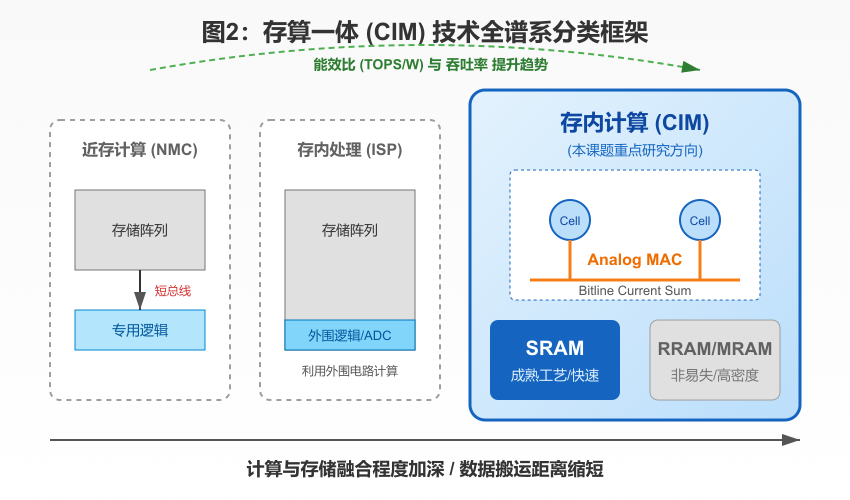
\includegraphics[width=0.8\textwidth]{figures/2.png}
\end{figure}

在国际研究中，基于新型非易失存储器（如 RRAM）交叉阵列的模拟 CIM/处理器近存储方案曾是重要热点，其核心优势在于可在交叉阵列中天然执行向量-矩阵乘法（VMM），以高并行度实现 CNN 的核心算子加速\cite{15}\cite{17}\cite{18}\cite{19}。典型代表包括 ISAAC（利用交叉阵列实现原位模拟算术以加速 CNN）以及 PRIME（将神经网络计算映射到 ReRAM 主存的 PIM 架构）等工作，这些研究表明将乘加“搬进存储阵列”在架构上可显著提升并行度与降低数据搬运成本。\cite{17}\cite{18} 同时，PUMA 等可编程 memristor 加速器进一步探索了在新型存储介质上实现更可编程的推理加速路径。\cite\cite{19} 但总体来看，模拟 CIM 往往需要 ADC/DAC 等外围电路并面临器件非理想性、噪声、精度与可校准性等挑战，高精度/多比特实现的系统开销与可靠性成为持续研究焦点。\cite{4}\cite{15}


除交叉阵列外，面向通用存储体系的“近存储/存内计算”也形成了多条路线，例如利用 DRAM 或 Cache 等商品化存储结构实现批量位运算或位串行加速，从而在不完全依赖新型器件的前提下提高数据就地处理能力。\cite{20}\cite{21}\cite{22} 例如 Ambit 利用 DRAM 的特性实现大规模位运算加速，Neural Cache 则探索在 Cache 内以位串行方式加速 DNN 计算，FloatPIM 进一步面向训练场景讨论了高精度需求下的 PIM 加速方式。\cite{20}\cite{21}\cite{22} 这类研究从体系结构角度强调“将计算靠近数据”的思想，并推动了从“仅优化算术单元”向“优化数据路径与存储层级协同”的范式转变。\cite{4}\cite{20}\cite{21}


在电路与工程实现层面，基于标准 CMOS 工艺的 SRAM-CIM 因其速度、成熟度与数字设计流程兼容性而成为当前研究与产业化的重要路线之一。\cite{5}\cite{12}\cite{14} SRAM-CIM 的关键问题之一是如何在保持阵列高并行度的同时支持多比特/符号数乘加，并控制外围电路（如累加、移位、感测/转换等）的面积与功耗开销。\cite{5}\cite{12} 针对多比特 MAC，已有多项芯片级宏单元工作给出了可参考的实现范式，例如：在 28nm 工艺下实现 8b MAC 的 SRAM-CIM 宏单元（展示了在 SRAM 宏中执行多比特 MAC 的可行性），以及支持 Signed-INT8、并强调 ADC-less（无 ADC）方向的 SRAM-CIM 宏单元工作等。\cite{8} 另有基于时间域（time-domain）思路实现 8b-MAC 的 SRAM-CIM 宏单元研究，表明通过不同的感测/编码与累加策略可在延迟、吞吐与能效之间做权衡。 同时，面向边缘侧推理的可配置位宽（1–8 bit）SRAM-CIM unit-macro 也显示出“在同一宏单元中支持多精度”的趋势，有利于适配不同模型的精度-能效需求。\cite{23}


更进一步，研究趋势正从“单个 CIM 宏单元验证”走向“可重构/可编程的数字 CIM 处理器与系统级加速器”，以提升可综合性、PVT 稳健性以及与 SoC/编译映射的适配能力。\cite{12}\cite{14}\cite{24}\cite{25} 例如，Tu 等在 ISSCC 报道了支持 BF16 与 INT8 的可重构数字 CIM 处理器，并强调统一 FP/INT 流水与阵列内乘法实现方式；其后续 ReDCIM 工作进一步在 JSSC 上从处理器形态给出统一 FP/INT 的数字 CIM 设计与加速思路。\cite{24}\cite{25} 同期也出现面向 Transformer/注意力工作负载的数字 CIM 加速研究，如 TranCIM、MulTCIM 等，体现出 CIM 技术从早期偏 CNN 的算子加速逐步扩展到更广泛模型形态，并结合稀疏性与重构模式在吞吐与能效上继续挖掘空间。\cite{26}\cite{27}


在算法侧，为了在保证精度的同时降低硬件复杂度与带宽压力，Int8 量化推理已成为工业界与学术界常用的落地路径之一。\cite{6} Jacob 等工作提出的整数算术推理量化方法表明，通过合理的 scale/zero-point 等量化参数与校准/训练策略，可在较小精度损失下使用整数算术完成推理，为硬件采用 Int8 数据通路提供了明确依据。\cite{6} 此外，PACT（激活裁剪）与 LSQ（学习步长量化）等研究进一步从训练与量化参数学习角度改善量化精度与稳定性，推动“量化策略—硬件实现”协同优化成为重要方向。\cite{28}\cite{29} 因而，对于面向工程实现的 CIM 阵列，如何在架构层面高效支持 Signed-INT8 的乘加、累加位宽管理、溢出/饱和与量化输出接口，已成为连接算法可用性与硬件可落地性的关键问题。\cite{5}\cite{6}\cite{12}


综合来看，国内外 CIM 研究呈现出以下发展趋势：第一，技术路线从“模拟/新型器件主导”逐步扩展为“模拟与全数字并行发展”，并更强调标准 CMOS 工艺兼容、可综合与可验证性，以降低工程落地门槛。\cite{4}\cite{12}\cite{14}\cite{24} 第二，算子与精度从早期偏低比特/位运算逐步走向多比特 MAC，尤其是与实际推理高度相关的 Signed-INT8，同时通过 ADC-less、时间域/数字逻辑等方式降低外围电路开销与提升稳健性。\cite{8}\cite{9}\cite{12}\cite{23} 第三，应用负载从 CNN 拓展到 Transformer/多模态与稀疏计算，CIM 加速器更强调重构性、数据流调度与系统级映射能力。\cite{26}\cite{27} 第四，从研究验证方式看，除芯片宏单元测试外，越来越需要体系结构层面的可复现验证与性能评估方法（包括 RTL/FPGA 原型验证、资源/频率/吞吐/延迟评估等），以支撑架构取舍与工程设计闭环。\cite{12}\cite{16}


因此，在已有研究基础上，仍存在值得进一步研究的空间：如何在“支持 Signed-INT8、多比特 MAC、低外围开销、可综合可验证”之间取得更优平衡，并形成可复用的阵列架构与验证平台，以服务于边缘视觉推理等典型场景。\cite{5}\cite{6}\cite{12}\cite{24} 本课题拟以数字 SRAM-CIM 阵列架构为核心，围绕数据通路、控制调度与 FPGA 验证建立工程闭环，从而在现有多比特 SRAM-CIM 宏单元与系统级落地需求之间提供可参考的架构设计与验证范式。\cite{5}\cite{12}\cite{24}

\section{研究内容}
\subsection{研究目标和可量化指标}
本课题面向YOLO、SSD等目标检测推理中占主导的卷积/点积（GEMM）算子，开展支持Signed-INT8的数字SRAM-CIM阵列架构设计，并完成RTL实现、功能仿真、FPGA综合部署与板级验证，形成“架构—RTL—验证—评估”的工程闭环。\cite{10}\cite{11}\cite{3} 研究对象覆盖权重在SRAM阵列内存储、阵列内实现乘法/部分积生成、片上（阵列内/阵列外）分层累加、以及与整数推理一致的舍入/饱和与重定标输出等关键环节。\cite{4}\cite{5}\cite{12}\cite{6}


为保证工程可验收性，拟建立如下可量化指标体系：


（1）功能正确性：在模块级与系统级测试中，与软件整数参考模型逐元素一致；覆盖Signed-INT8负数运算、极值输入、累加溢出与饱和等边界情形，确保补码语义与量化语义一致。\cite{6}\cite{28}\cite{29}


（2）性能模型与可测量性：给出cycle级吞吐/延迟估算方法（含装载、计算、写回阶段），并在FPGA上用性能计数器对关键阶段cycle数进行测量与校核，保证报告中性能结论可复现。\cite{3}\cite{24}\cite{25}


（3）可扩展与可配置：阵列维度M×N、tile数量、bit-plane展开度、累加层级与输出位宽等关键参数可配置，以支持不同卷积层形态（Cin/Cout、K×K、输出像素块大小）映射与设计空间探索。\cite{12}\cite{23}\cite{24}


（4）资源与时序约束：统计并分析FPGA实现的LUT/FF/BRAM（及必要时DSP）占用与最高工作频率Fmax，给出在资源受限条件下的并行度选型原则与关键路径规避策略。\cite{24}\cite{25}


（5）验证完整性：形成覆盖“单元—阵列—系统”三级回归的测试体系，包含随机向量、定向边界用例、关键断言与覆盖统计，确保工程实现达到可交付质量。\cite{12}\cite{16}

\subsection{总体架构与技术路线}
（1）技术路线选择与依据：针对内存墙与数据搬运能耗问题，本课题采用“数字SRAM-CIM阵列”路线，将点积计算尽量靠近权重存储位置，以减少权重反复读取与跨层级搬运开销，并利用阵列并行性提高吞吐与能效。\cite{2}\cite{4}\cite{5} 相比依赖模拟外设（如ADC/DAC）的方案，数字化路线更易与标准RTL流程对接，更适合在FPGA上进行快速原型验证与工程迭代；多篇综述与趋势工作指出SRAM-CIM正向更高精度、多位宽与系统级可重构方向发展，数字化与可综合化是重要演进方向之一。\cite{12}\cite{13}\cite{14} 同时，已有多比特（8b）与Signed-INT8的SRAM-CIM宏单元研究，以及可重构数字CIM处理器研究，为本课题的多比特与符号数实现可行性提供了直接支撑。\cite{7}\cite{8}\cite{9}\cite{24}\cite{25}

\begin{figure}[H]
	\centering
	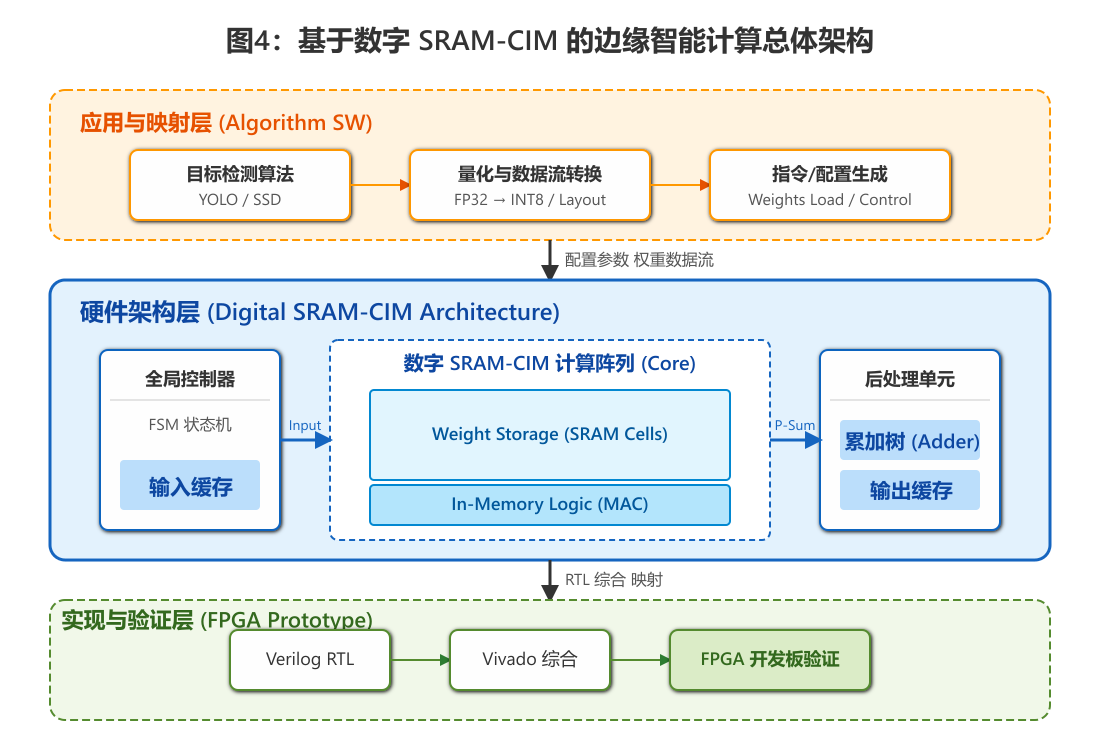
\includegraphics[width=0.8\textwidth]{figures/4.png}
\end{figure}



（2）从卷积/点积到阵列运算的映射：将卷积层通过im2col或直接滑窗展开为“激活向量×权重矩阵”的点积序列；权重矩阵以Signed-INT8形式写入SRAM阵列，激活向量以片上缓冲/流式输入方式提供，并按bit-plane或小组位宽广播至阵列列/行；阵列内完成按位与/异或/选择等数字逻辑的部分积生成与局部累加，随后通过分层累加形成输出通道的psum，再进行舍入/饱和与重定标得到INT8或更高位宽输出。\cite{3}\cite{6} 该映射方式与CNN加速器数据流优化的基本思想一致，可将大量MAC并行化并降低访存压力。\cite{3}\cite{5}

\begin{figure}[H]
	\centering
	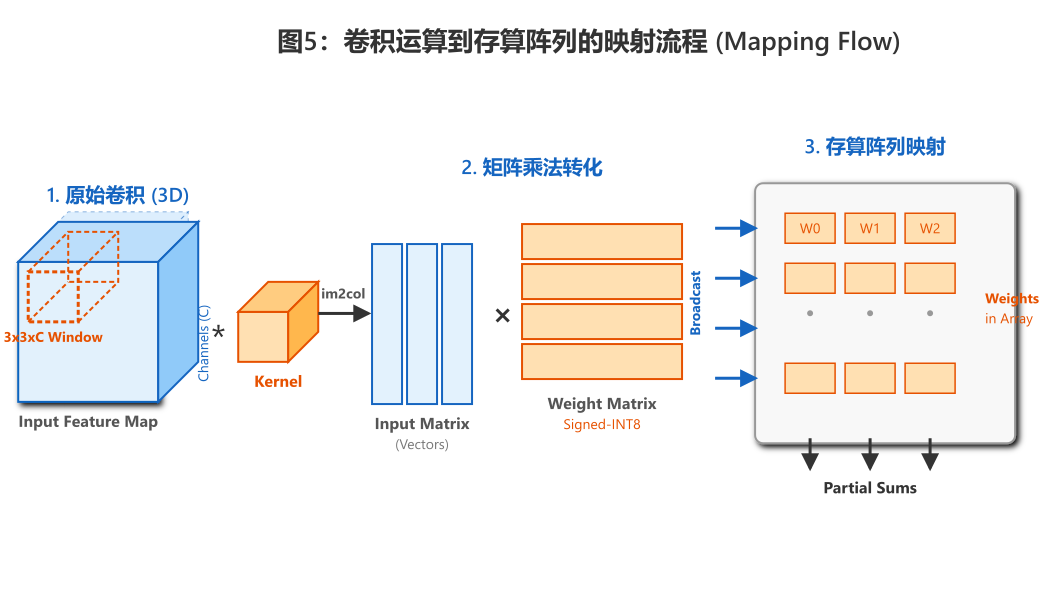
\includegraphics[width=0.8\textwidth]{figures/5.png}
\end{figure}



（3）系统级接口与工程实现思路：整体架构采用“输入缓冲—CIM阵列/Tile阵列—分层累加与量化输出—输出缓冲”的流水式组织；控制器负责权重装载、激活调度、bit-plane循环与写回；在FPGA实现中利用BRAM/URAM缓存权重块与激活块，必要时提供AXI-like流式接口用于测试向量装载与结果回读，保证板级验证可操作。\cite{16}\cite{24}\cite{25}


\subsection{关键模块设计}
为实现端到端可综合验证，本课题将架构拆分为可复用、可组合的RTL模块，并明确数据流/控制流关系。总体模块包括：权重存储与装载模块（Weight SRAM/Loader）、激活缓冲与广播模块（Act Buffer/Broadcast）、CIM基本单元与阵列模块（CIM Cell/Array/Tile）、分层累加模块（Local/Global Accumulator）、量化/重定标模块（Requant/Sat/Round）、控制与调度模块（FSM/Scheduler）、顶层接口与测量模块（Top/IF/Counter）。\cite{12}\cite{16}


（a）Signed-INT8 CIM基本单元设计：

\begin{figure}[H]
	\centering
	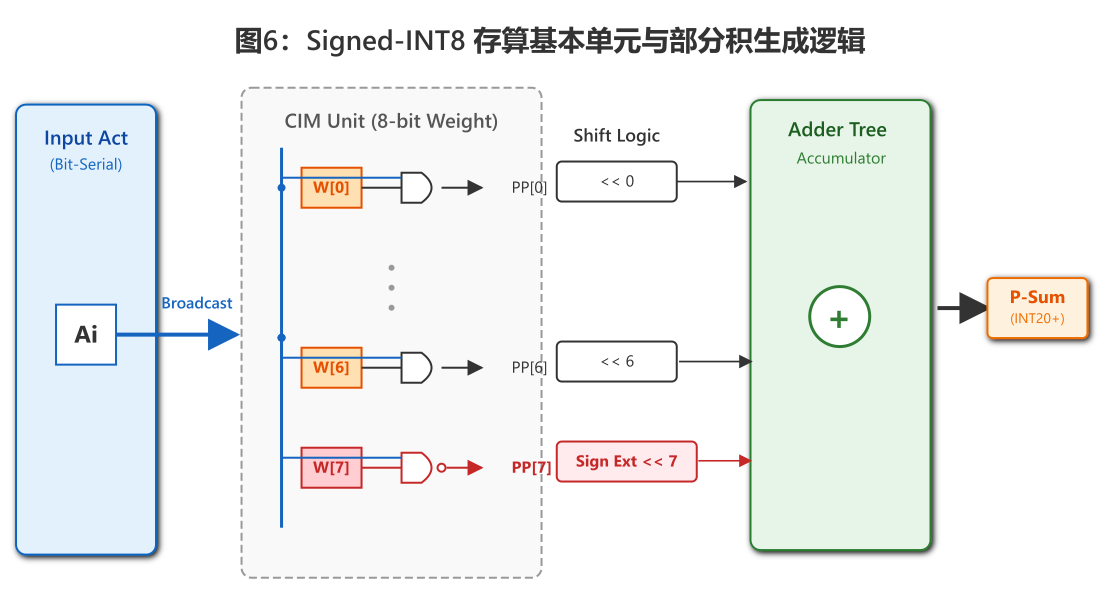
\includegraphics[width=0.8\textwidth]{figures/6.png}
\end{figure}



基本单元以SRAM存储Signed-INT8权重，采用二进制补码表示，保证与主流整数推理一致。\cite{6} 乘法实现策略优先采用“bit-plane部分积生成+移位累加”的数字化表达：激活按位（或按2–4位小组）广播，权重按位参与生成部分积；符号位通过符号扩展或修正项并入累加链路，保证负数乘法的等价性与可验证性。\cite{8}\cite{20} 该类多比特MAC在SRAM-CIM宏中已有实现与验证，表明在阵列内部进行多比特运算并输出可累加的部分和在工程上可行；同时，Signed-INT8宏与ADC-less方向进一步提示可通过数字逻辑与合适编码降低外围开销。\cite{7}\cite{8}\cite{9}


（b）阵列/Tile组织与并行度参数：




采用参数化M×N阵列（如M行对应输出通道并行度，N列对应输入通道/展开维度并行度），并支持多Tile拼接以扩展吞吐；提供并行度旋钮，包括：阵列维度（M、N）、bit-plane展开度（一次并行处理的bit数）、tile数量、以及输出聚合宽度。\cite{12}\cite{23}\cite{24}

\begin{figure}[H]
	\centering
	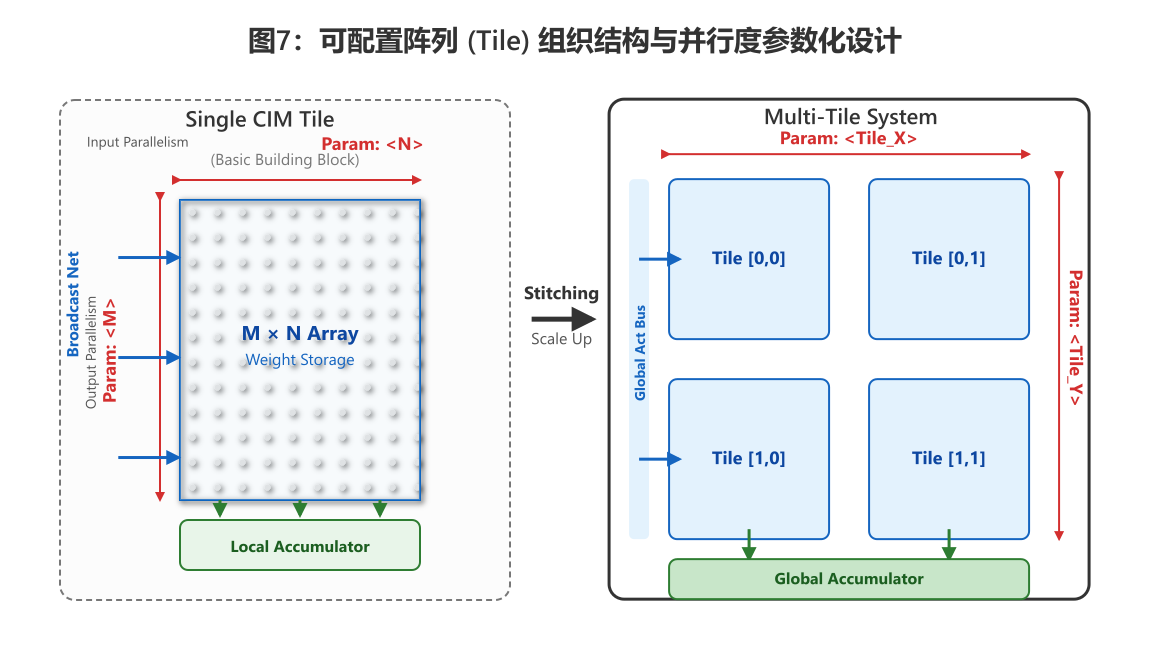
\includegraphics[width=0.8\textwidth]{figures/7.png}
\end{figure}

在数据流上，激活通过广播网络送达列侧，权重驻留于SRAM，阵列输出局部psum经收集网络送入累加层级；该组织与多精度SRAM-CIM宏的可配置思想一致，便于在FPGA资源约束下进行折中选型。\cite{23}\cite{5}


（c）累加与精度管理（psum规划、舍入/饱和与重定标）：


由于卷积点积长度随Cin与核大小变化，psum位宽需按最坏情况规划，设置保护位（guard bits）以避免中间溢出；累加可采用“tile内局部累加+跨tile全局累加”的分层结构，减少单级加法树深度并利于时序收敛。\cite{3}\cite{24}\cite{25} 输出阶段提供可配置的舍入与饱和逻辑，将高位宽psum映射回INT8或指定输出位宽；重定标过程遵循整数推理常用量化形式（scale/zero-point或对称signed），量化参数支持配置加载，以便与模型校准/量化训练策略一致。\cite{6}\cite{28}\cite{29}

\begin{figure}[H]
	\centering
	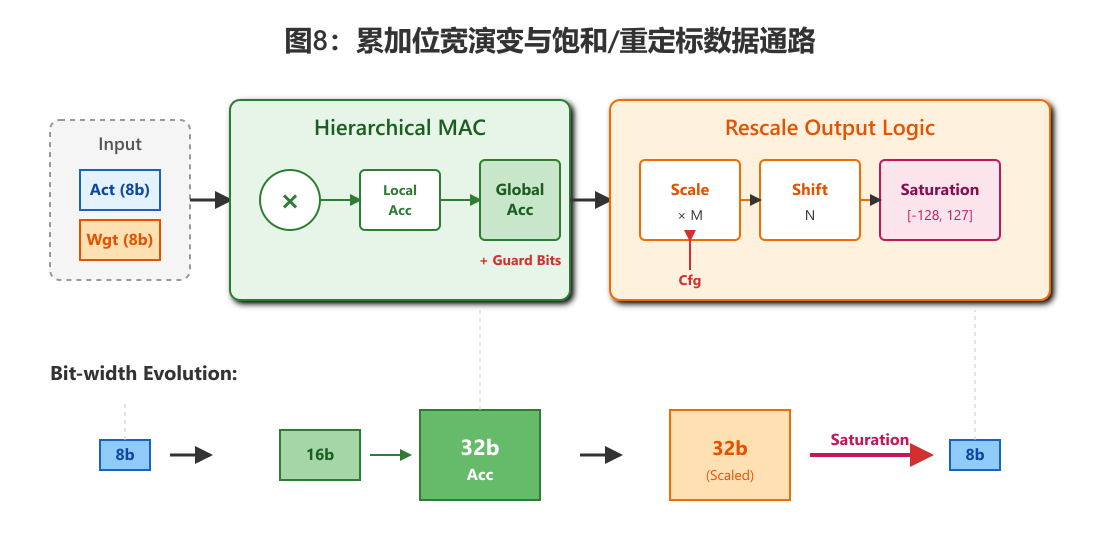
\includegraphics[width=0.8\textwidth]{figures/8.png}
\end{figure}


（d）数据通路与控制调度（可流水、可缓冲）：


控制器以FSM实现权重装载、激活块装载、bit-plane循环、计算与写回；在时序上将“部分积生成—局部累加—全局累加—量化输出”划分为可流水的阶段，必要时引入双缓冲（ping-pong）以隐藏装载延迟并提高阵列利用率。\cite{3}\cite{24} 为便于性能评估，建立cycle级模型：装载阶段与计算阶段分别计数，计算阶段进一步分解为bit-plane迭代次数与阵列并行度关系，从而得到吞吐与延迟的可解释表达式，并在FPGA上通过计数器验证模型有效性。\cite{24}\cite{25}


（e）FPGA顶层集成与可测量接口：


顶层集成包括：BRAM/URAM权重缓存与激活缓存、可选AXI-stream/存储映射寄存器接口、测试向量装载与输出捕获模块、以及性能计数器与调试端口（如ILA可观测信号）。\cite{16}\cite{24} 通过“离线生成测试向量→板上装载→运行→回读对比”的流程实现功能闭环，并可进一步在板上实现小规模卷积层映射作为端到端示例。\cite{10}\cite{11}\cite{3}


\subsection{创新点}
（1）面向FPGA原型的可综合、可参数化数字SRAM-CIM阵列RTL框架：现有多比特与Signed-INT8 SRAM-CIM研究多以固定宏单元形态展示，难以直接用于阵列规模、并行度与数据流的体系结构探索。\cite{7}\cite{8}\cite{23} 本课题提出模块化、参数化RTL抽象（阵列维度、bit-plane展开、累加层级等），并在FPGA上进行周期级可观测验证；数字CIM处理器工作表明系统级数字化CIM的工程实现路径可行。\cite{24}\cite{25}\cite{12} 预期收益是实现从“宏单元启发”到“可复现架构评估”的桥接，提高设计迭代效率与工程可交付性。\cite{12}\cite{16}


（2）Signed-INT8友好的部分积/符号处理与外围开销协同优化：多位宽运算中符号处理与外围累加往往成为开销来源。\cite{5}\cite{12} 本课题在补码语义下设计符号修正项与部分积生成协同策略，探索借鉴ADC-less Signed-INT8宏与数字CIM乘法/编码思路，减少有效部分积数量或降低累加深度。\cite{8}\cite{24} 可行性由Signed-INT8 SRAM-CIM宏与多比特MAC宏的实践共同支撑。\cite{8}\cite{7}\cite{9} 预期收益是在维持Signed-INT8正确性的前提下降低关键路径压力与外围逻辑规模，提升FPGA可实现频率与阵列利用率。\cite{24}\cite{25}


（3）与整数推理一致的分层累加—舍入/饱和—重定标链路：工程落地中软硬一致性是决定可用性的关键，而多比特累加与输出量化容易引入语义偏差。\cite{6} 本课题提出层次化累加与位宽管理策略，并实现可配置的舍入/饱和与重定标接口，对齐整数推理流程，同时兼容PACT、LSQ等量化训练/校准思想以提升泛化适配能力。\cite{6}\cite{28}\cite{29} 多精度SRAM-CIM宏与可重构数字CIM系统表明多位宽路径与重构机制具备工程实现基础。\cite{23}\cite{25} 预期收益是降低模型迁移成本、提高结果可解释性与可复现性。\cite{12}\cite{16}


（4）“软件golden—RTL—FPGA”三层一致的验证与评估方法学：现有CIM研究常以芯片测试或高层仿真给出结论，体系结构级的可复现评估流程相对不足。\cite{12}\cite{16} 本课题建立以整数推理规则为核心的软件参考模型，并将cycle计数、资源统计与板级对比纳入统一流程；该思路与系统级数字CIM研究的工程化趋势一致。\cite{24}\cite{25}\cite{12} 预期收益是形成可复用的评测基准与报告模板，支撑后续架构对比与创新点量化论证。\cite{4}\cite{12}
\subsection{验证与评估方法}


\begin{figure}[H]
	\centering
	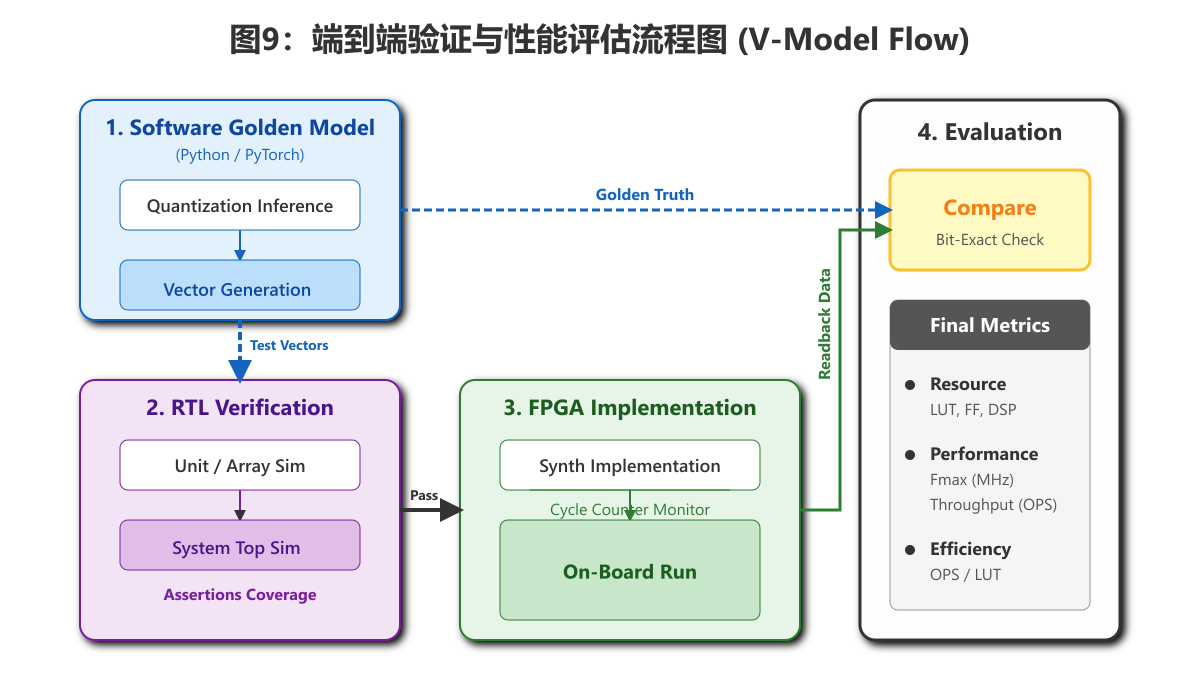
\includegraphics[width=0.8\textwidth]{figures/9.png}
\end{figure}

（1）RTL验证计划：采用“单元级→阵列级→系统级”的分层验证策略。单元级针对Signed乘法、符号扩展/修正、舍入/饱和与重定标模块进行定向用例与随机回归；阵列级验证并行度、bit-plane循环与累加层级一致性；系统级验证包含权重装载、激活装载、计算与写回全流程。\cite{12}\cite{16} 测试向量覆盖负数、全1/全0、最大最小、随机分布与点积长度变化导致的累加极值；关键接口加入断言（如补码一致性、溢出触发条件、握手时序）并统计覆盖率，以提高工程可靠性。\cite{12}\cite{6}


（2）软件golden模型：以整数算术推理为准，构建bit-accurate参考模型，包含（可选）对称或含zero-point的量化形式、scale参数、累加位宽与最终重定标；量化策略与PACT、LSQ等方法的核心思想保持兼容，使得硬件结果可与量化后网络推理语义一致。\cite{6}\cite{28}\cite{29}


（3）FPGA验证流程：完成综合与时序收敛后，上板执行“向量装载—运行—结果回读—对比”闭环，结合在线计数器记录装载/计算/写回cycle数，核对cycle模型；必要时通过分级寄存与流水化降低关键路径并提升Fmax。\cite{24}\cite{25}


（4）评估指标：资源（LUT/FF/BRAM/URAM/DSP）、最高频率Fmax、cycles/op、吞吐估算（ops/s）与端到端延迟；在不同阵列参数与bit-plane配置下形成设计空间点，给出资源—性能折中曲线与推荐配置。\cite{24}\cite{25}\cite{16} 可选地实现一个小规模卷积层映射作为证明性案例，展示与目标检测工作负载的关联与端到端正确性。\cite{10}\cite{11}\cite{3}
\subsection{预期成果与交付物}
本课题预期形成可直接验收的工程交付物：①完整RTL代码（含参数化CIM基本单元、阵列/Tile、分层累加、量化/重定标、控制与顶层接口）；②系统化验证平台（testbench、随机/定向用例集、断言与覆盖统计、自动化回归脚本）；③FPGA工程与板级验证流程文档（向量装载/回读、性能计数器、调试信号说明）；④性能评估报告（资源、频率、吞吐、延迟、配置对比）与映射示例；⑤开题与论文所需的架构图、数据流图、时序/吞吐模型说明等配套材料，满足工程设计类毕设“代码+验证+评估”要求。\cite{12}\cite{16}\cite{24}\cite{25}

\section{研究计划及进度安排}
%\begin{itemize}
本课题研究周期预计为 16 周，涵盖文献调研、架构设计、RTL 开发、FPGA 验证及论文撰写五个阶段，具体安排如下：


第 1 - 2 周：文献调研与方案论证 深入研读数字 SRAM-CIM 及量化推理相关文献 ；确定 Int8 补码乘加运算的逻辑实现方案；完成系统级架构草图绘制与数据流模型初步建立 。


第 3 - 4 周：关键算法模型与 Golden 模型构建 使用 Python/C++ 构建符合 Int8 补码语义的 Bit-accurate 软件参考模型；确定舍入（Round）、饱和（Sat）与重定标（Requant）的数学映射关系，为后续 RTL 验证提供比对标准 。


第 5 - 8 周：硬件描述语言（HDL）设计与模块建模 采用 Verilog/SystemVerilog 开发 CIM 基本单元、M×N 阵列及分层加法树 ；设计支持权重/激活双缓冲加载的控制状态机（FSM）；完成各子模块的定向用例测试。


第 9 - 11 周：系统集成、仿真与时序优化 集成顶层架构，开展“单元级→阵列级→系统级”的分层仿真回归 ；针对 FPGA 平台进行时序约束分析，通过插入流水线寄存器等手段优化关键路径，确保 Fmax 达到预期指标。


第 12 - 14 周：FPGA 综合部署与性能评估 在开发板上完成板级调试；利用性能计数器记录实际运行 Cycle 数，验证吞吐率与延迟模型 ；统计 LUT、BRAM 等资源占用，完成设计空间探索与性能评估报告。


第 15 - 16 周：毕业论文撰写与成果交付 整理设计文档、测试覆盖率报告及 RTL 代码库；完成开题报告中定义的各项量化指标对齐 ；撰写并完善毕业论文，准备最终答辩。
%\end{itemize}

\begin{figure}[H]
	\centering
	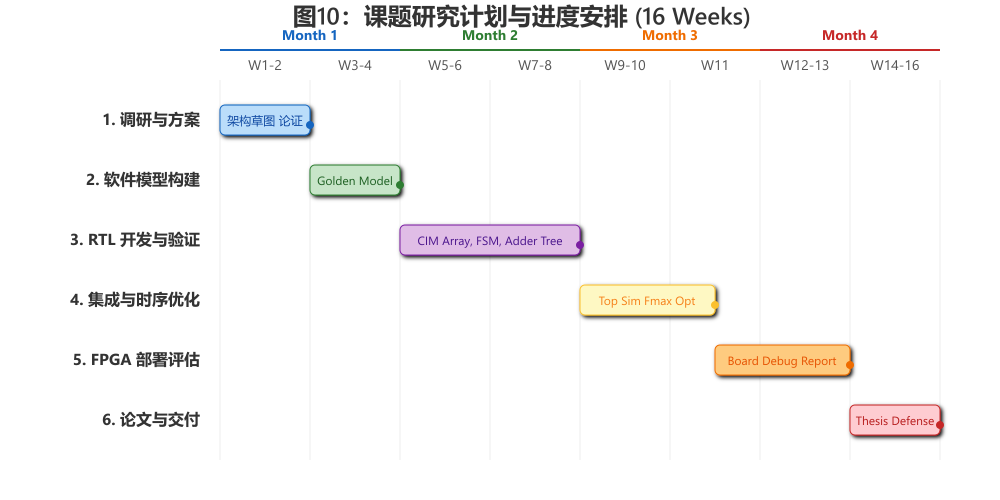
\includegraphics[width=0.8\textwidth]{figures/10.png}
\end{figure}


\section{参考文献}
% ieeetr 引用顺序　plain 首字母顺序　alpha 缩写标识
\nocite{*}
\printbibliography[heading=none]
\end{document}
